\chapter{Конструкторский раздел}
В данном разделе будут рассмотрены требования к программе и алгоритмы визуализации сцены.

\section{Общий алгоритм решения поставленной задачи}
\begin{enumerate}
	\item загрузить объекты сцены;
    \item отобразить объекты сцены;
	\item позволить пользователю изменять параметры и показать результат в реальном времени.
\end{enumerate}


\section{Шаги графического конвейера}

Рассмотрим работу графического конвейера.

\begin{figure}[H]
	\begin{center}
		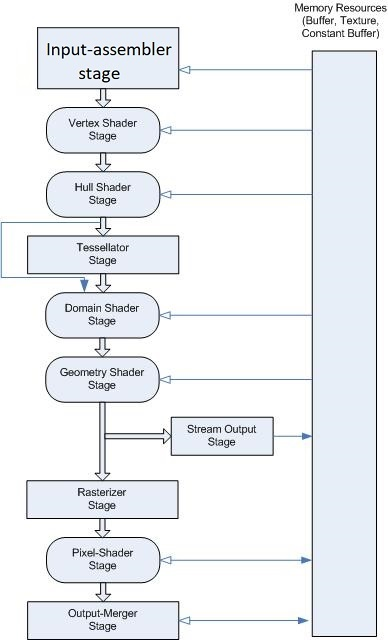
\includegraphics[scale=0.88]{img/conveer.jpg}
	\end{center}
	\captionsetup{justification=centering}
	\caption{Работа графического конвейера}
	\label{img:konv}
\end{figure}

Для простоты реализации, и учитывая факт, что большинство из этих шагов недоступны разработчикам, было принято решение ограничить их число. 


\begin{enumerate}
 \item шаг отбрасывания невидимых объектов (работает на ограничивающих сферах на процессоре);
 \item шаг тесселяции;
 \item шаг формирования z-буфера;
 \item шейдер вершин;
 \item шаг отбрасывания целиком невидимых поверхностей;
 \item шаг растеризации и шейдер пикселей.
\end{enumerate}


Шаги шейдера вершин, отбрасывания целиком невидимых поверхностей, а также растеризации объединены в один. Это связано с производительностью реализации.
Рассмотрим шаги по порядку.

\section{Шаг отбрасывания невидимых объектов}

Отбрасывание полностью невидимых объектов происходит на процессоре. Для этого используется пирамида видимости, представленная на 
рисунке \ref{img:frustum_view}. Это обусловлено использованием перспективной проекции. Пирамида является усеченной и состоит из 6 граней.
Эти грани можно аналитически описать с помощью уравнений плоскости. Создается оболочка, содержащая трехмерный объект.
Для определения видимости объекта решается задача нахождения расположения оболочки относительно граней пирамиды видимости.
Виды оболочек показаны на рисунке \ref{img:frustum_casing}.

\begin{figure}[H]
	\begin{center}
		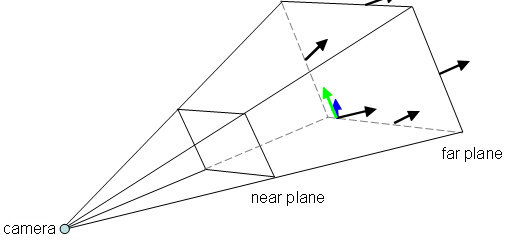
\includegraphics[scale=0.88]{img/frust_1.png}
	\end{center}
	\captionsetup{justification=centering}
	\caption{Пирамида видимости}
	\label{img:frustum_view}
\end{figure}

\begin{figure}[H]
	\begin{center}
		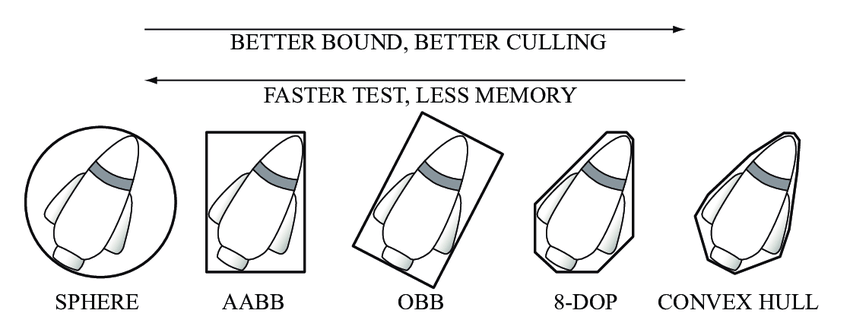
\includegraphics[scale=0.5]{img/frust_casing.png}
	\end{center}
	\captionsetup{justification=centering}
	\caption{Виды оболочек, левее - используют меньше ресурсов, правее - предоставляют большую точность}
	\label{img:frustum_casing}
\end{figure}

Для быстродействия и простоты имплементации была выбрана сферическая оболочка. В данном случае возможны три варианта 
расположения сферы относительно плоскости, показанные на рисунке \ref{img:frustum_sphere}. Для того чтобы объект считался полностью невидимым, его
сфера должна находиться по невидимую сторону от любой из граней усеченной пирамиды. Иначе, объект считается видимым, или частично видимым, и происходит вызов его отрисовки.

\begin{figure}[H]
	\begin{center}
		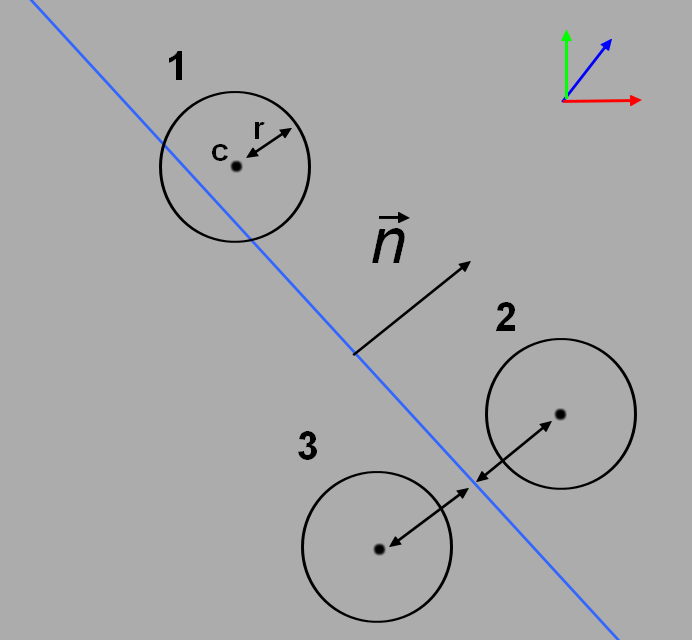
\includegraphics[scale=0.5]{img/frust_3.png}
	\end{center}
	\captionsetup{justification=centering}
	\caption{Варианты расположения сферы относительно плоскости}
	\label{img:frustum_sphere}
\end{figure}

\subsection{Асинхронный анализ виртуальной геометрии}

Данный шаг, в совокупности с последующим, аналогичен тесселляции в реальной графическом конвейере.
Виртуальной назовем геометрию, которой не существует в статическом описании модели на файле. Виртуальная геометрия генерируется процедурно, во время выполнения программы.

В этом шаге считается площадь каждой грани отрисовываемой модели (прошедшей фильтрацию по области видимости).
Грани, площадь которых превышает порог, рекурсивно разбиваются на подграни виртуальной геометрии в следующем шаге.
При этом, на данном шаге вычисляется количество виртуальных граней, чтобы заранее выделить необходимый объем видеопамяти при построении геометрии.
Таким образом, увеличивается количество отрисовываемых треугольников. Теоретически, уменьшение количества тоже возможно, но выходит за рамки работы.

Используется несколько анализаторов моделей, каждый из которых работает асинхронно. Параллелизм идет по граням отдельной модели.
Количество анализаторов задано статически, и превышает количество виртуальных моделей. Таким образом все виртуальные модели анализируют.

\begin{figure}[H]
	\centering
	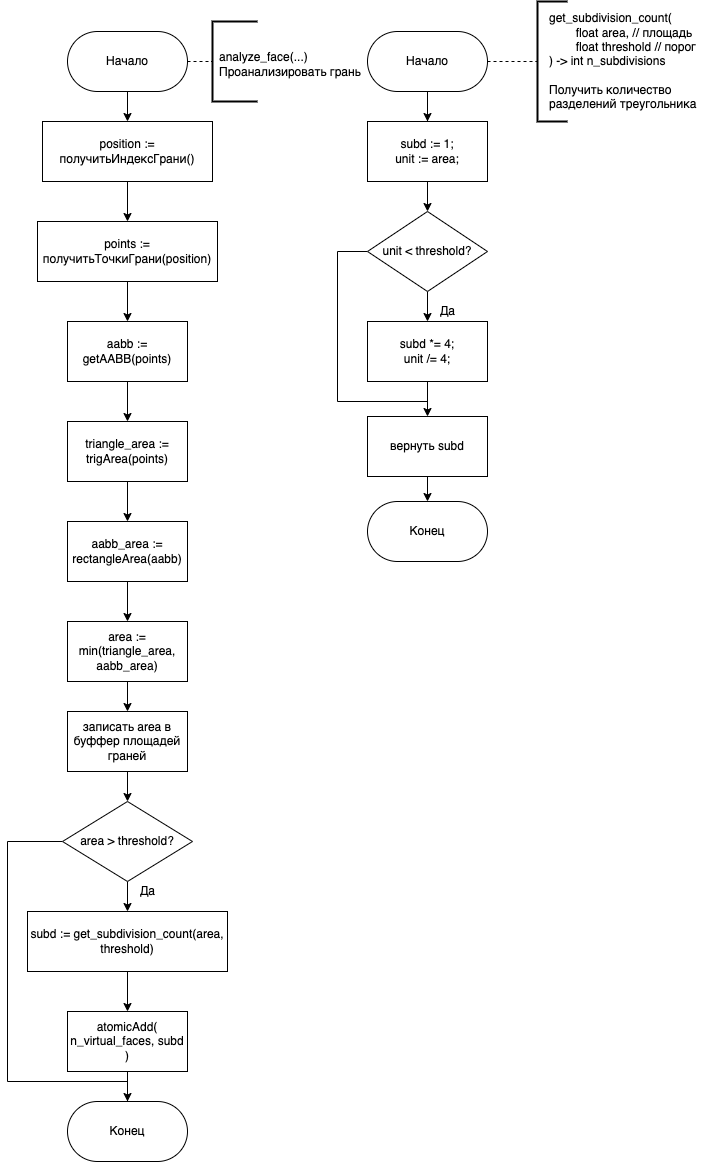
\includegraphics[height=0.95\textheight]{img/diagrams-vgeom_analyzer.drawio.png}
	\caption{Разработка алгоритма анализа геометрии}
	\label{fig:geom_analyzer_kernel}
\end{figure}


\subsection{Создание или обновление виртуальных объектов}

Выделяются буферы для вершин, граней и дополнительных векторов нормалей, текстур.
Новые треугольники копируются в отдельную модель, называемую виртуальной. Логически, это отдельная модель, которая инъектируется в множество отрисовываемых моделей на этапе отрисовки.
Грани, заменяемые новой моделью, помечаются как неактивные, и не обрабатываются.

\begin{figure}[ph!]
	\centering
	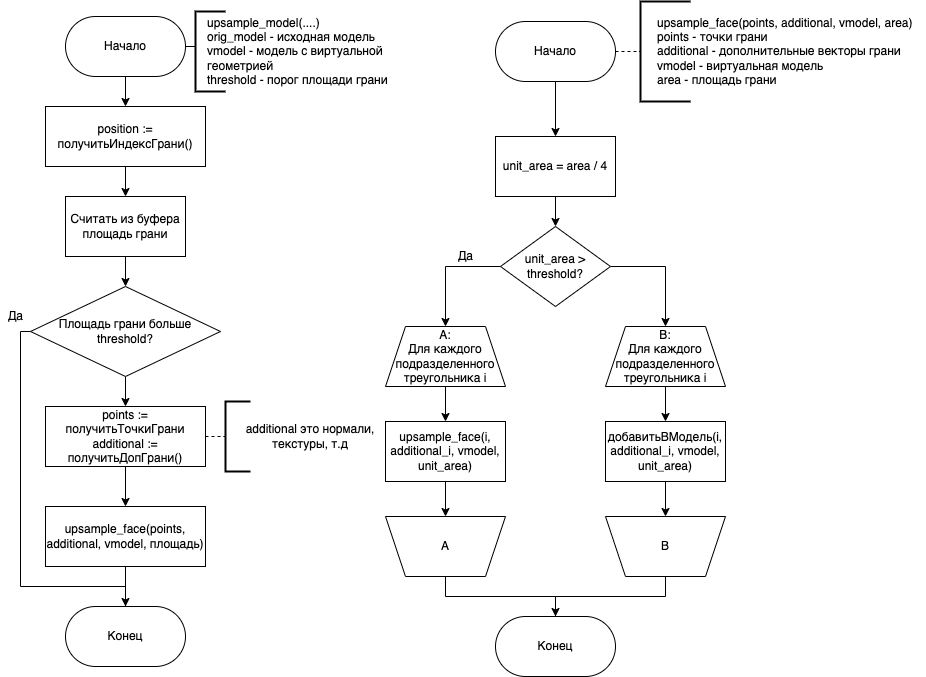
\includegraphics[width=1\linewidth]{img/diagrams-vgeom_upsampler.drawio.png}
	\caption{Разработка алгоритма создания виртуальной геометрии} 
	\label{fig:vgeom_create_kernel}
\end{figure}


\section{Алгоритм z-буфера}

Алгоритм z-буфера был выбран из за его чрезвычайной параллельности и, как следствие, быстродействия. Реальный графический конвейер использует именно этот алгоритм. 

Для демонстрации проблем, возникших в реализации курсового проекта, можно рассмотреть подход к разработке алгоритма Z-буфера.

Можно реализовать его тремя способами:

\begin{itemize}
	\item параллельность ведется по граням моделей. При этом приходится использовать операцию AtomicCAS, блокирующую шину памяти.
	\item параллельность ведется по пикселям на экране. При этом в цикле рассматривается множество граней модели.
	\item модификация первого подхода, но несколько моделей отрисовываются в отдельные буферы, которые потом параллельно объединяются.
\end{itemize}

Были проведены тесты, в которых последний подход оказался самым быстродействующим. Отчасти это связано с отсутствием конфликтов в банках памяти, при выполнении неделимой операции atomicCAS к разным буферам.
С подобными проблемами прошлось сталкиваться во всех аспектах реализации.

\begin{figure}[H]
	\begin{center}
		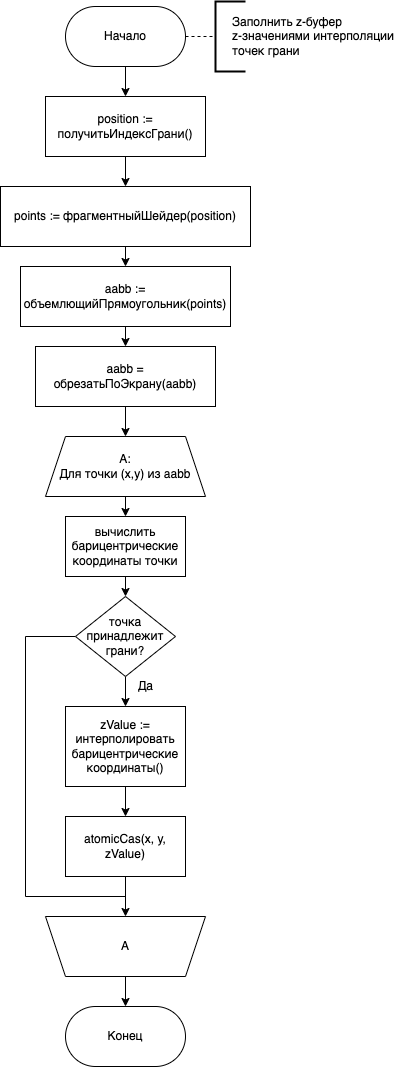
\includegraphics[scale=0.5]{img/diagrams-zfiller.drawio.png}
	\end{center}
	\captionsetup{justification=centering}
	\caption{Разработка алгоритма z-буфера}
	\label{img:z_buffer}
\end{figure}


Как было оговорено выше, модели на сцене равномерно распределяются между z-буферами. Всего буферов $ 2^n $ штук. В реализации n=32.

После обработки каждой, происходит слияние z-буферов в один, используя алгоритм параллельной редукции. Идея его работы показана на 
рисунке \ref{img:parallel_reduce}. Параллелизм происходит по пикселям буфера. Два буфера на каждом шаге обрабатываются независимо (асинхронно) от других.

\begin{figure}[H]
	\begin{center}
		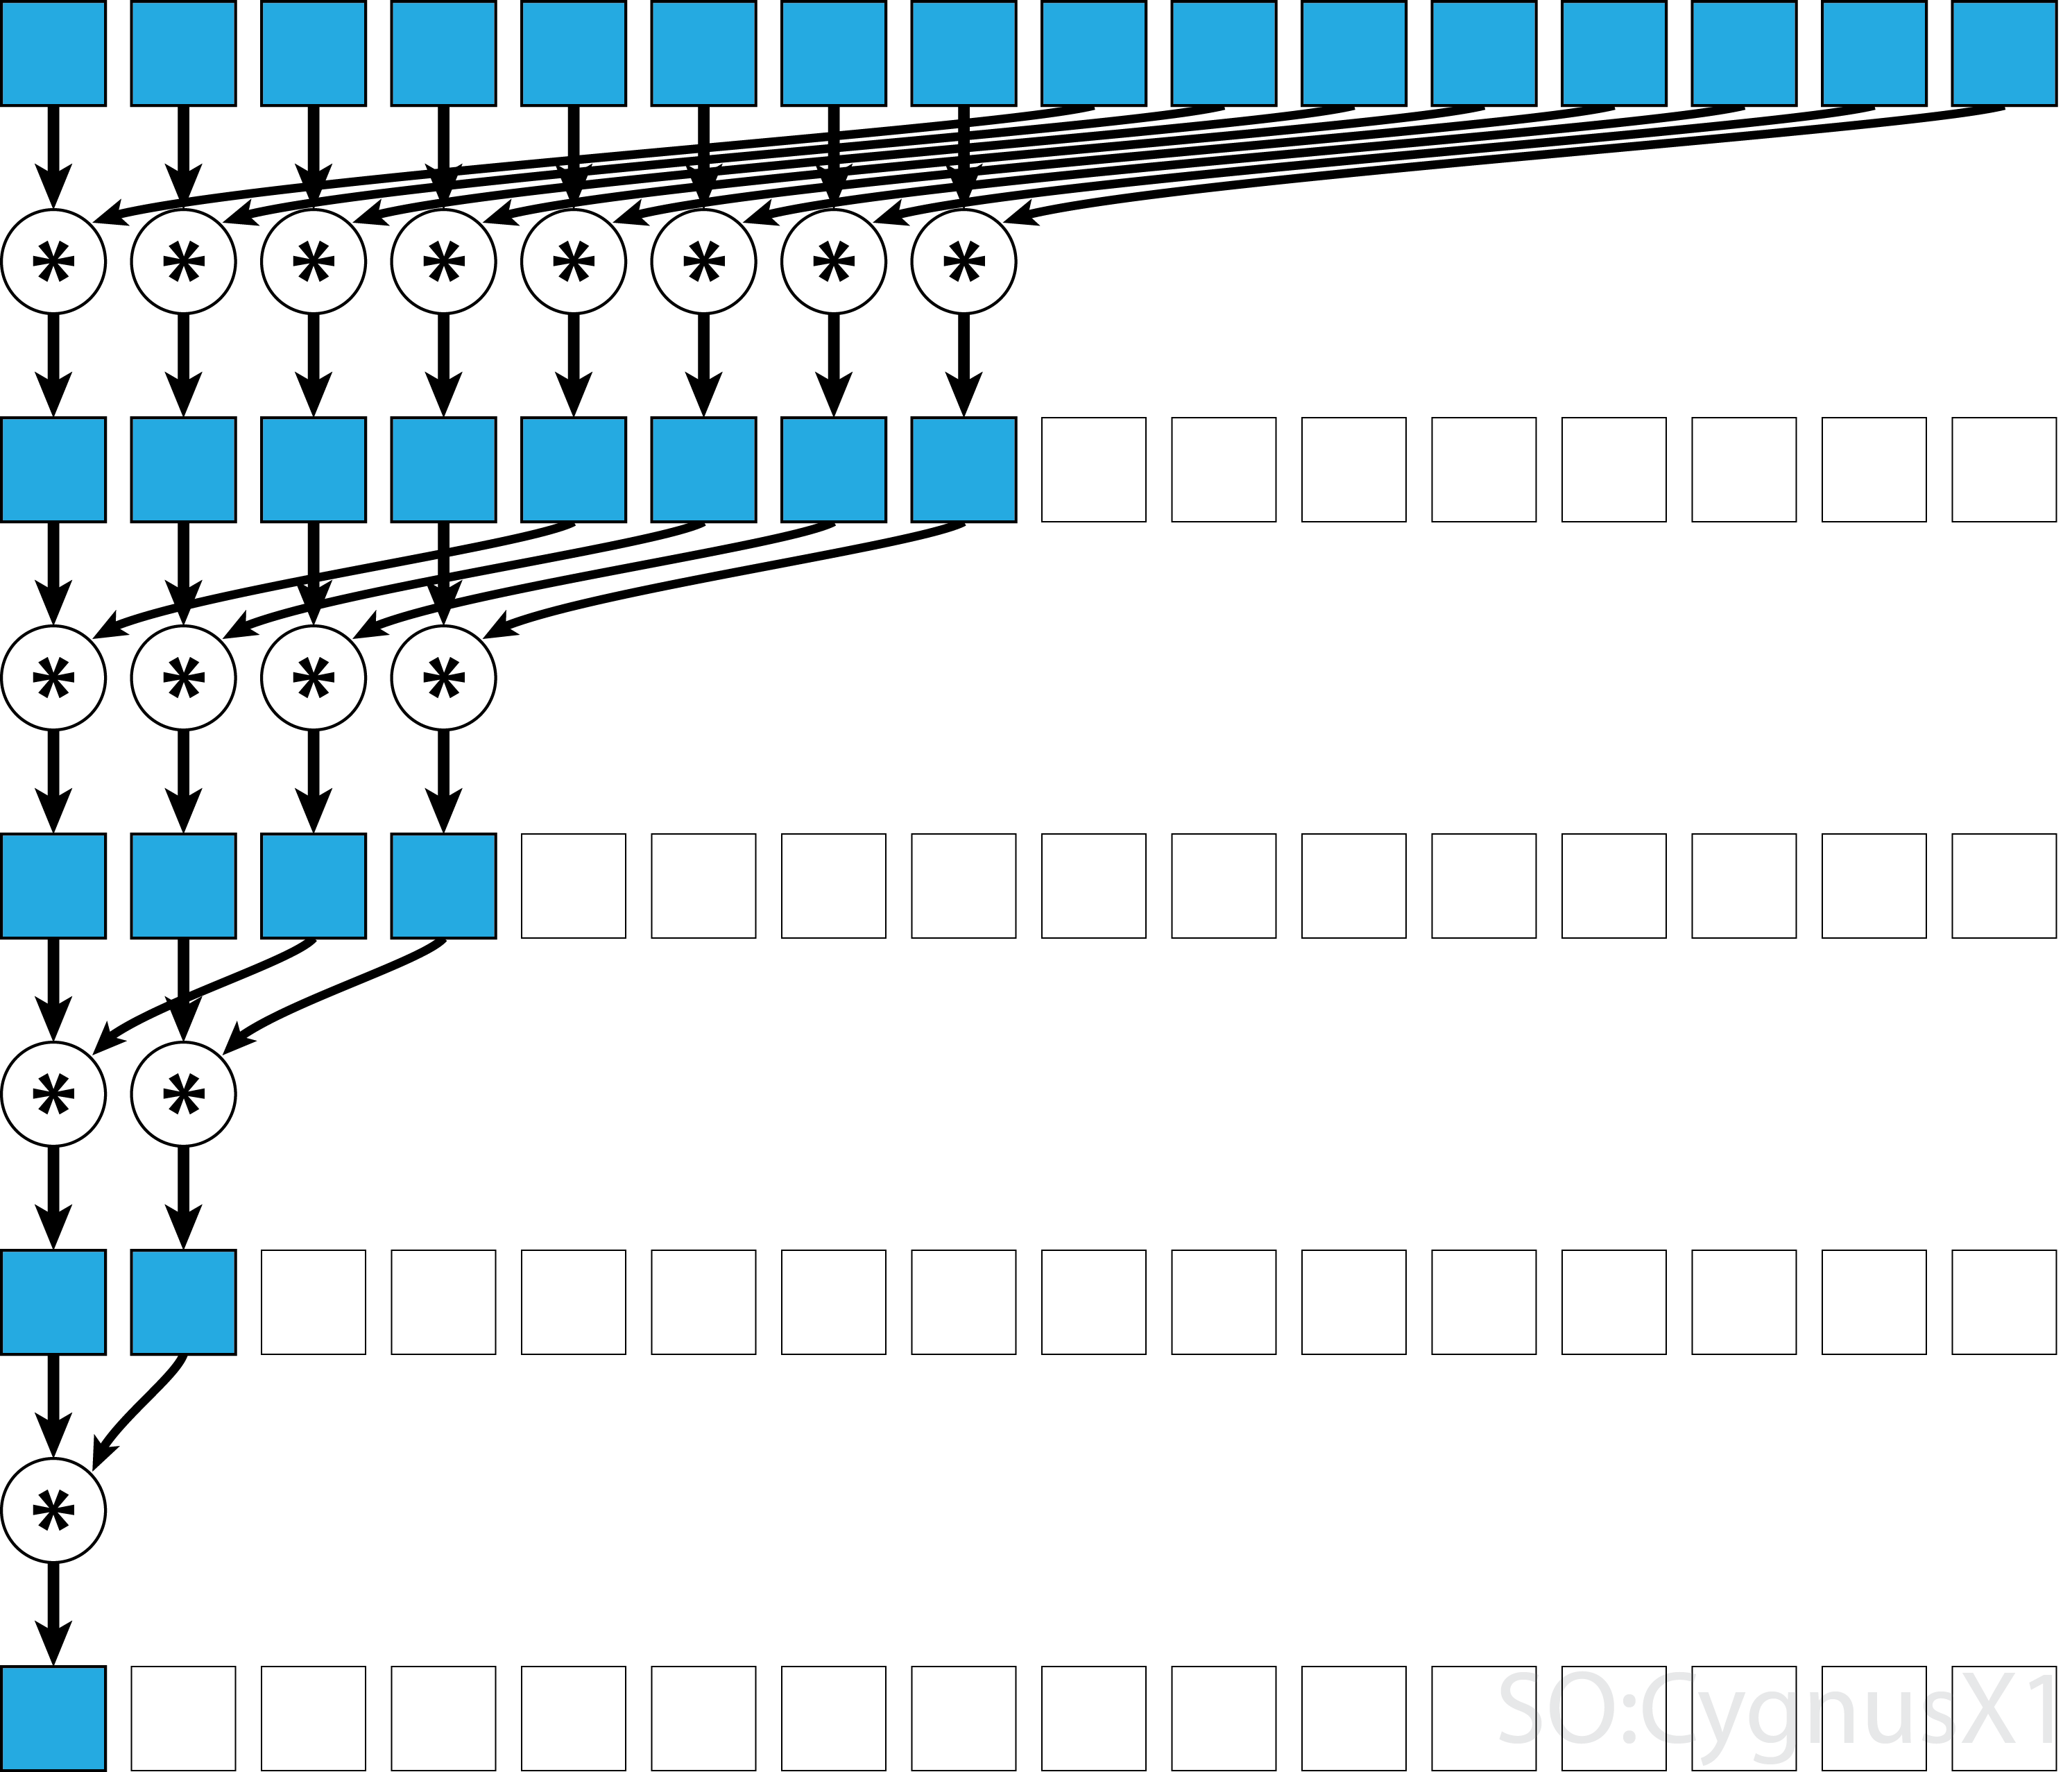
\includegraphics[scale=0.3]{img/parallel_reduction.png}
	\end{center}
	\captionsetup{justification=centering}
	\caption{Идея работы алгоритма параллельной редукции}
	\label{img:parallel_reduce}
\end{figure}

\section{Отрисовка объектов}

После заполнения z-буфера, происходит отрисовка объектов, используя алгоритм растеризации.

Каждая грань отрисовывается в отдельном потоке. При этом используется информация z-буфера. Если интерполированное значение проецированного пиксела равно значению z-буфера,
такрй пиксел выводится на растр.

\begin{figure}[H]
	\centering
	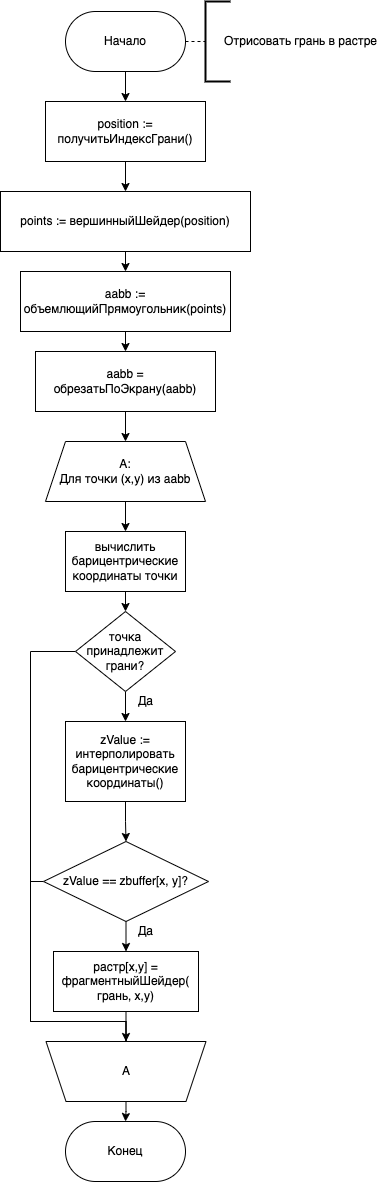
\includegraphics[height=0.95\textheight]{img/diagrams-rasterizer.drawio.png}
	\caption{Разработка алгоритма растеризации}
	\label{fig:diagram_count}
\end{figure}


\section{Выбор используемых типов и структур данных} 

Для разрабатываемого ПО необходимо реализовать следующие типы и структуры данных.
\begin{enumerate}
	\item Сцена - список объектов.
	
	\begin{verbatim}
	class Scene {
		private:
		std::vector<SceneObject> models{}; // Модели
		std::shared_ptr<Camera> camera{};  // Камера
		glm::vec3 light_dir{0, 0, 1};      // Направление освещения
		int id_counter = 0;                // id последнего зарегистрированного объекта
		int scene_id = 0;                  // версионный вектор лампорта сцены. свидетельствует об изменениях.
		int time = 0;                      // время сцены
		bool sorted = false;               // отсортированы ли объекты по id

		// callback, вызывается каждый тик
		std::function <void(Scene &)> on_update = [](Scene &) {}; 
	\end{verbatim}

	\item Объекты сцены
	
		\begin{Verbatim}[tabsize=4]
struct ModelRef {
	TextureRef texture{};
	glm::vec3 *vertices{}; // вершины
	glm::vec3 *normals{};
	glm::vec2 *textures{};
	// индекс текстуры для грани
	glm::ivec3 *textures_for_face{};
	glm::ivec3 *faces{}; // грани
	// кол-во вершин, граней, текстур
	int n_vertices = 0;
	int n_faces = 0;
	int max_texture_index = 0;
	int id = 0;
	// объемлющая сфера для куллинга
	Sphere *bounding_volume{};

	RegisteredShaders shader = RegisteredShaders::Default;

	bool is_virtual = false; // является ли модель виртуальной
};
	\end{Verbatim}
		
	\item Текстура
	\begin{Verbatim}
struct TextureRef
{
	int x = 0; // ширина
	int y = 0; // высота 
	int n = 0; // кол-во каналов
	uchar3 *data{}; // данные текстуры
	[[nodiscard]] __device__ uchar3 get_uv(float u, float v) const;
};
	\end{Verbatim}

	\item Шейдер.
	\begin{Verbatim}
struct BaseShader
{
	glm::mat4 projection;
	glm::mat4 view;
	glm::mat4 model_matrix;

	ModelRef &model;
	const DrawCallBaseArgs &base_args;

	glm::vec3 pts[3]{};
	glm::vec3 normals[3]{};
	glm::vec2 textures[3]{};
	glm::vec3 light_dir{};
	glm::vec2 screen_size{};
	int position = 0;

	float4 vertex(int iface, int nthvert, bool load_tex);


	bool fragment(glm::vec3 bar,
	 			uint &output_color,
				float z_value);
};
	\end{Verbatim}
	\item Математические абстракции:
	\begin{enumerate}
		\item вектор;
		\item сфера;
		\item луч;
		\item плоскость;
	\end{enumerate}
\end{enumerate}


\section*{Вывод}
В данном разделе были подробно рассмотрены алгоритмы, которые будут реализованы, приведены схемы алгоритмов для решения поставленной задачи и описаны используемые структуры.
